\section{Seismic}

\section{Thermal}

\section{Laser Frequency}

\section{Laser Intensity}

\section{Electronics}

\section{Residual Gas}

\section{Noise Budget}

\begin{figure}[htbp]
	\centering
		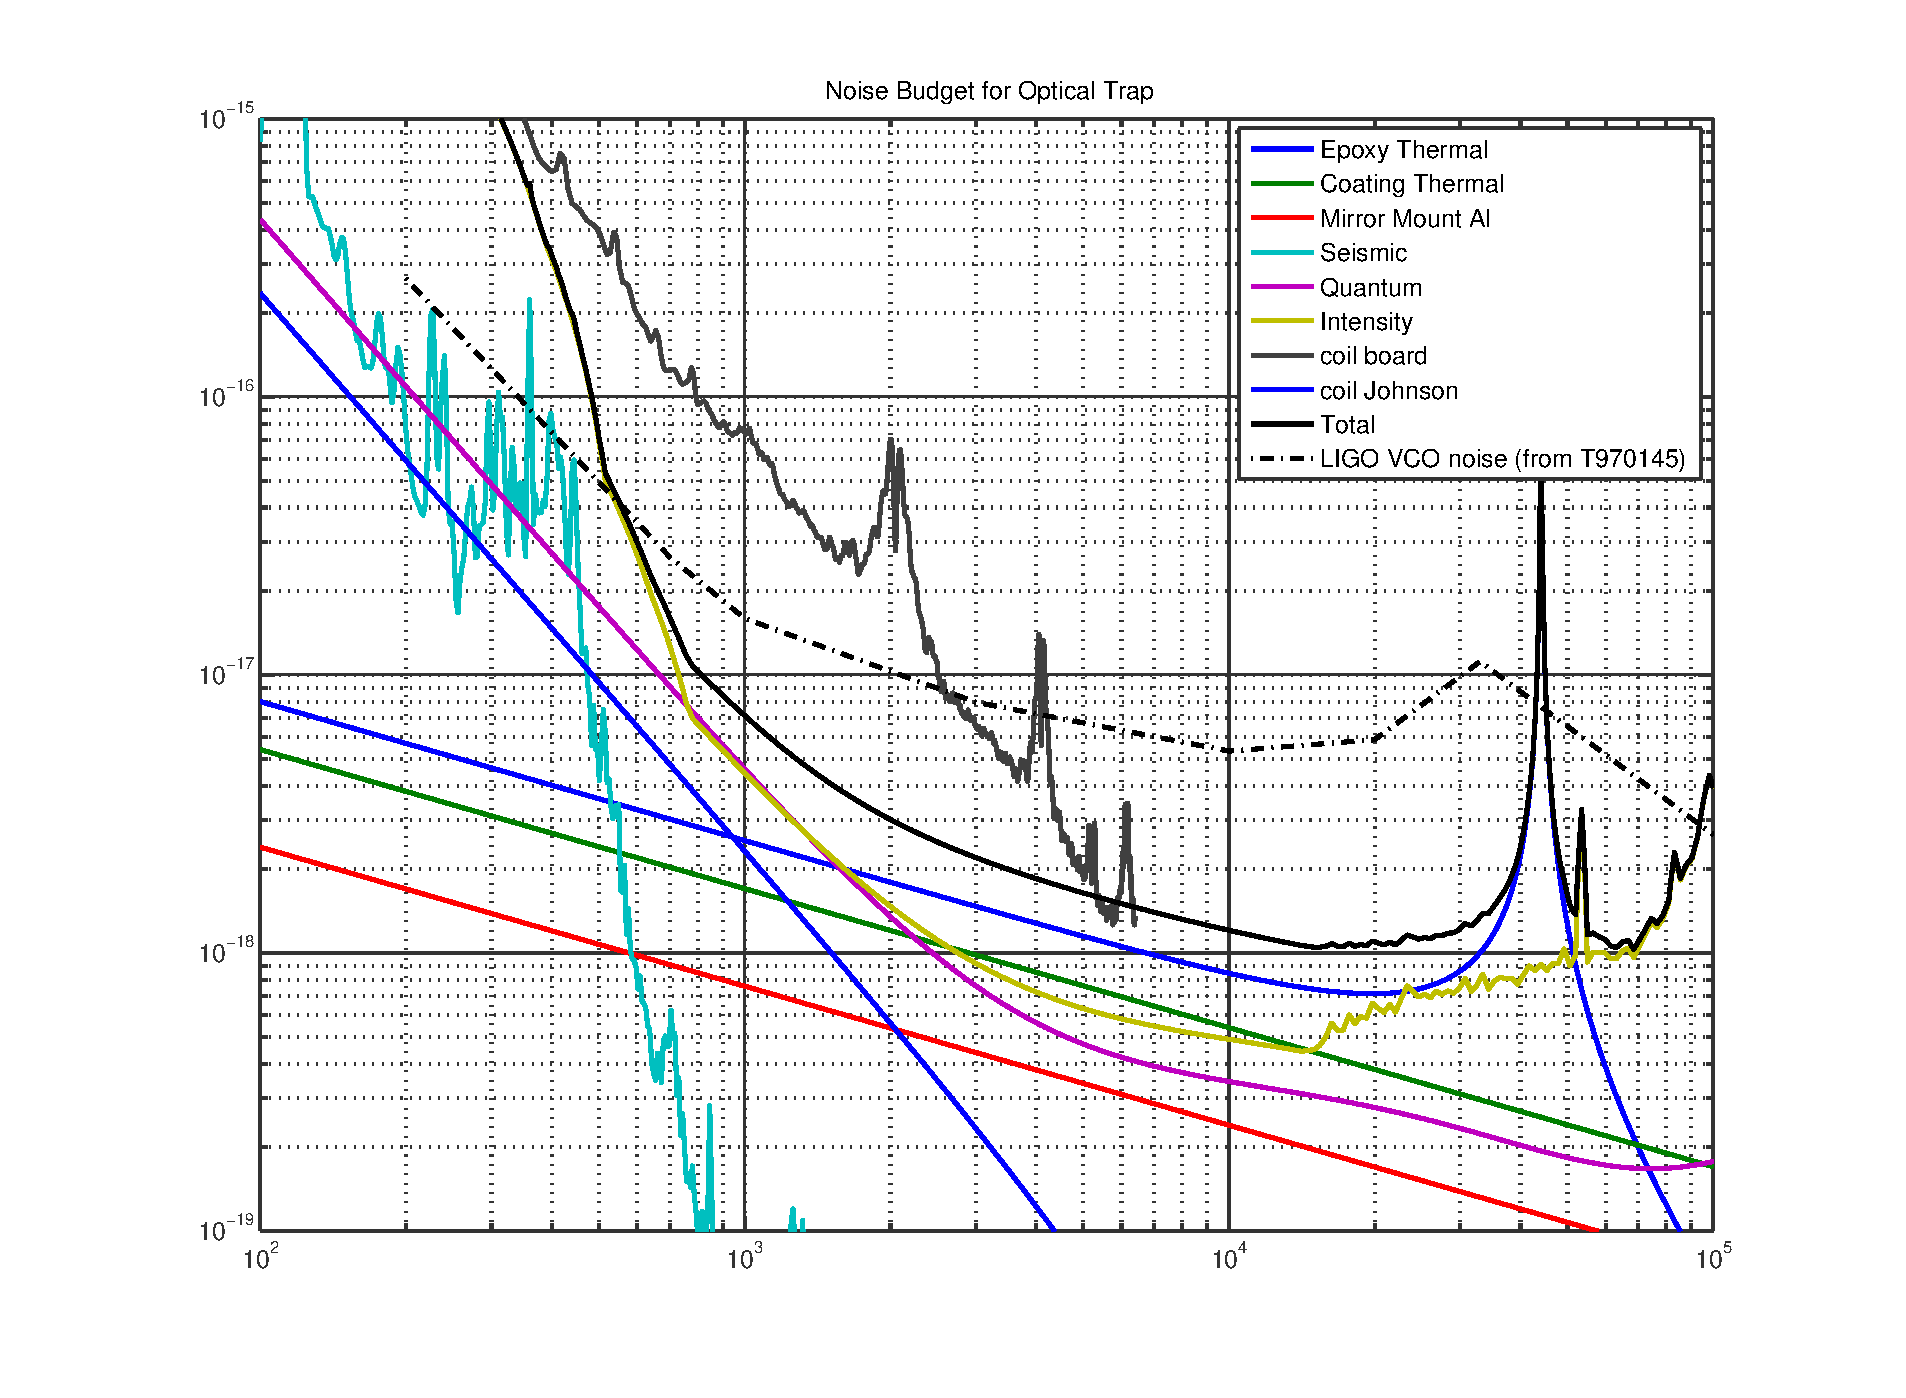
\includegraphics[width=15cm]{./figures/noise_budget.eps}
	\caption[Noise Budget]{Noise budget}
	\label{fig:noise_bud}
\end{figure}

\begin{figure}[htbp]
	\centering
		\includegraphics[width=15cm]{./figures/NoiseBudgetBoard.pdf}
	\caption[Noise Budget Board]{Noise budget with coil driver board noise}
	\label{fig:noise_bud_brd}
\end{figure}

\section{Vacuum Requirements for Optical Trap}

It is desired to have an understanding of limits of vacuum gas constituents for the in-vacuum experiment. From the LIGO DCC we have a few documents that describe the process that went into understanding the problem for 2 4km long Fabry-Perot cavities. I will apply these techniques to a 10-30cm cavity.\\


\subsection{LIGO Vacuum Requirements}

The amplitude spectral density of the optical path length is given by,

\begin{align*}
\Delta L ( f ) = 4 \pi \left( \frac{2 L_0 p}{k T w_0 v_0} \right)^{1/2} a e^{- \pi f w_0 / v_0 }
\end{align*} \\


From *** the value for $4 \pi a \left( \frac{2}{k T w_0 L_0 v_0} \right)^{1/2} $ is $ 4.8 x 10^{-21} \left( \frac{R_x}{R_{H_2}} \right) $. Where $L_0 = 4000 \mathrm{m} $ and $ w_0 = 0.06 \mathrm{m} $. \\

For our purposes (single arm cavity) we will lose a factor of $ \sqrt{2} $. \\

We end up with a formula for amplitude spectral density in a one-arm cavity that is:

\begin{align*}
\Delta L ( f ) = 4 \pi \left( 5.3 \mathrm{x} 10^{-20} \right) \left(  \frac{R_x}{R_{H_2}} \right) \sqrt{\frac{ L_0 p}{ w_0 } } e^{- \pi f w_0 / v_0 }
\end{align*} \\

\subsection{Optical Trap}

Now, we insert parameters for the cavity. For the first look, I use the parameters defined in the project description: 0.3m cavity length, 0.2m radius of curvature for each mirror.
\todo{something},

If we operate at a pressure of 1e-6 Torr, no constituent gas can be greater than this. The following plot is of constituent gases at this pressure.

\begin{figure}[htbp]
	\centering
		\includegraphics[width=15cm]{./figures/trapgasnoise_1.png}
	\caption[Gas Noise Comparison]{Gas Noise for 1e-6 Torr}
	\label{fig:gas_noise1}
\end{figure}

If we have a residual gas analyzer that detects a minimum partial pressure of 5e-11 Torr:

\begin{figure}[htbp]
	\centering
		\includegraphics[width=15cm]{./figures/trapgasnoise_2.png}
	\caption[Gas Noise Comparison]{Gas Noise for 5e-11 Torr}
	\label{fig:gas_noise2}
\end{figure}

\section{Epoxy Thermal Noise}

Brownian thermal noise estimates for epoxy joints are gotten from basic application of the fluctuation-dissipation theorem. The form that we start with is,
\begin{align*}
S_{x^2}(f) = \frac{4 k_B T}{\omega^2} \Re(Z^{-1}), 
\end{align*}
where $Z$ is the impedance, $F / v$. The force equation that we use is of the form,
\begin{align*}
F_{\mathrm{ext}} = m \ddot{x} + k x,
\text{where k is a complex number}, (1 + i \phi)
\end{align*}

\section{Derivation}

\begin{align*}
d_n = d(t-\tau_n)
\end{align*} \\

\begin{align*}
d_n = d \left( t - \frac{(2n -1)}{c} L_0 - d_1 - \sum_{l=2}^{n} 2 d_l \right)
\end{align*} \\

